\documentclass[conference]{IEEEtran}

\usepackage{hyperref}
\usepackage{pgfgantt}
\usepackage{graphicx}
\graphicspath{{src/}}

\title{Waveform and Transceiver Design for Dual-Mode MIMO Wireless Information and Power Transfer}

\author{Supervisor: Dr Bruno Clerckx (b.clerckx@imperial.ac.uk)
    \\
    Student: Yang Zhao (yang.zhao18@imperial.ac.uk)}

\date{\today}

\begin{document}

\maketitle

\begin{abstract}
  In this research, we consider a dual-mode Multi-Input Multi-Output (MIMO) wireless information and power transfer (WIPT) system with multiple Energy Harvesters (EH). To that end, we aim to design a generic transceiver architecture where a sensor node dynamically switches between single-subband and multi-subband transmissions with proposed Mode Switching (MS) algorithm according to the received power level. For Frequency-Flat (FF) and Frequency-Selective (FS) channel, a single-tone amplitude and phase modulation will be combined with a novel tone-index multisine modulation that enables information transmission via subset index. At the receiver, a power splitter is introduced after each antenna to reallocate the received signal to different rectifiers for high energy conversion efficiency. The proposed algorithm jointly optimizes beamforming, power splitting and MS operation based on practical nonlinear EH models for single and multi-tone waveforms. Compared with existing strategies, it is expected to produce a larger rate-energy (R-E) region and operating range with lower computational complexity.
\end{abstract}

\section{Background}
A major problem for smart networks as Internet-of-Things (IoT) is the power source. Although batteries have removed the physical boundary for mobile devices, the limited working time and frequent recharging and replacement have become main restrictions for the development of wireless networks. Recently, with the significant reduction in power requirement of electronics, Simultaneously Wireless Information and Power Transfer (SWIPT) with Radio-Frequency (RF) signals has become a sustainable solution to power mobile devices while keeping them connected.

\section{Literature Review}
The possibility of SWIPT was first explored in \cite{R.Varshney2008}, where the pioneer defined a capacity-energy function and investigated the trade-offs for a frequency-flat (FF) Gaussian channel and typical binary channels. \cite{Grover2010} extended the research to frequency-selective (FS) channels. Both works are based on the ideal assumption that the entire received signal is used for individual Energy Harvesting (EH) and Information Decoding (ID). \cite{Zhang2013} proposed two practical receiver designs, namely \textit{Time Switching} (TS) that switches between EH and ID on time basis and \textit{Power Splitting} (PS) that splits the received signal into separate portions. However, the works before \cite{Clerckx2016} are mostly based on an oversimplified linear harvester model. Based on the Taylor expansion of the diode characteristic equation, the authors derived a tractable \textit{diode nonlinear model} for Wireless Power Transfer (WPT) to characterize the nonlinear behavior of the rectifier, and performed an adaptive multisine waveform design accordingly. It was demonstrated by circuit simulations that the rectifier nonlinearity brings significant gains to the harvested power and radically influences wireless system design. \cite{Clerckx2018} extended the work to SWIPT where a superposition of modulated information waveform and multisine power waveform is jointly optimized with the power splitting ratio, according to the Channel State Information (CSI) and rate requirements. It reported that harvester nonlinearity benefits the rate-energy (R-E) tradeoff and favors a different waveform, modulation, and input distribution. Nevertheless, the algorithms rely on iterative Geometric Programming (GP) optimization and the computational cost increases exponentially with the number of subbands. In comparison, \cite{Park2018} proposed a dual-mode SWIPT with an adaptive \textit{Mode Switching} (MS) algorithm to alternate between single-tone and multi-tone transmission. The former employs a multi-energy level signaling with Phase Shift Keying (PSK) for high rate communication, while the latter modulates the multisine waveform by Peak-to-Average Power Ratio (PAPR) for power-demanding applications \cite{Krikidis2019}. Nevertheless, it only considered the case with Single-Input Single-Output (SISO) and one energy harvester. A generic receiver architecture for Multi-Input Multi-Output (MIMO) was designed in \cite{Ma2019}, which demonstrated that using multiple rectifiers with proper beamforming and power allocation scheme can significantly improve the harvested power. However, it focused on WPT only and omitted the coupling among beamforming, transmit signal and power splitting factors discovered in \cite{Huang2017}.

\section{Aims and Objectives}
In this research, we aim to extend the dual-mode SWIPT in \cite{Park2018} to MIMO multi-harvester case and optimize the waveform through a joint design of beamforming, power splitting and MS operation, based on two nonlinear harvester models proposed in \cite{Boshkovska2015} and \cite{Clerckx2016}. We will investigate the relationship between the performance (achievable R-E region, bit error rate, outage probability) and configuration (number of antennas and rectifiers) for FF and FS channels.

\section{Method and Design}

\paragraph{System structure}

\begin{figure}
  \centering
    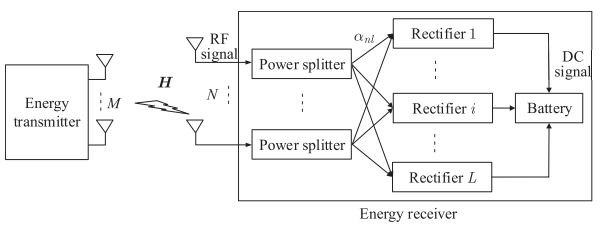
\includegraphics[width=0.45\textwidth]{system_architecture}
  \caption{System architecture of the proposed MIMO WIPT system \cite{Ma2019}}
  \label{fig:system_architecture}
\end{figure}

Consider a point-to-point MIMO WIPT system with $M$ transmitters, $N$ receivers, and $L$ rectifiers. Figure \ref{fig:system_architecture} illustrates the system structure from energy perspective. In the system, each receive antenna is followed by a splitter to determine the input power of the rectifiers. Specifically, when the received power level is relatively low, the splitters will combine all energy branches in one rectifier to enjoy the benefit of harvester nonlinearity. In contrast, when the power is sufficiently high, the components will be equally divided to avoid the saturation of diode breakdown region \cite{Clerckx2019}. The harvested power is then combined and stored in the battery.

\paragraph{Non-linear Energy Harvester Model}

A nonlinear EH model proposed in \cite{Boshkovska2015} whose parameters relies on curve fitting will be compared with the diode nonlinear model in \cite{Clerckx2016}.

\paragraph{Waveform Design and Transceiver Architecture}

\begin{figure}
  \centering
    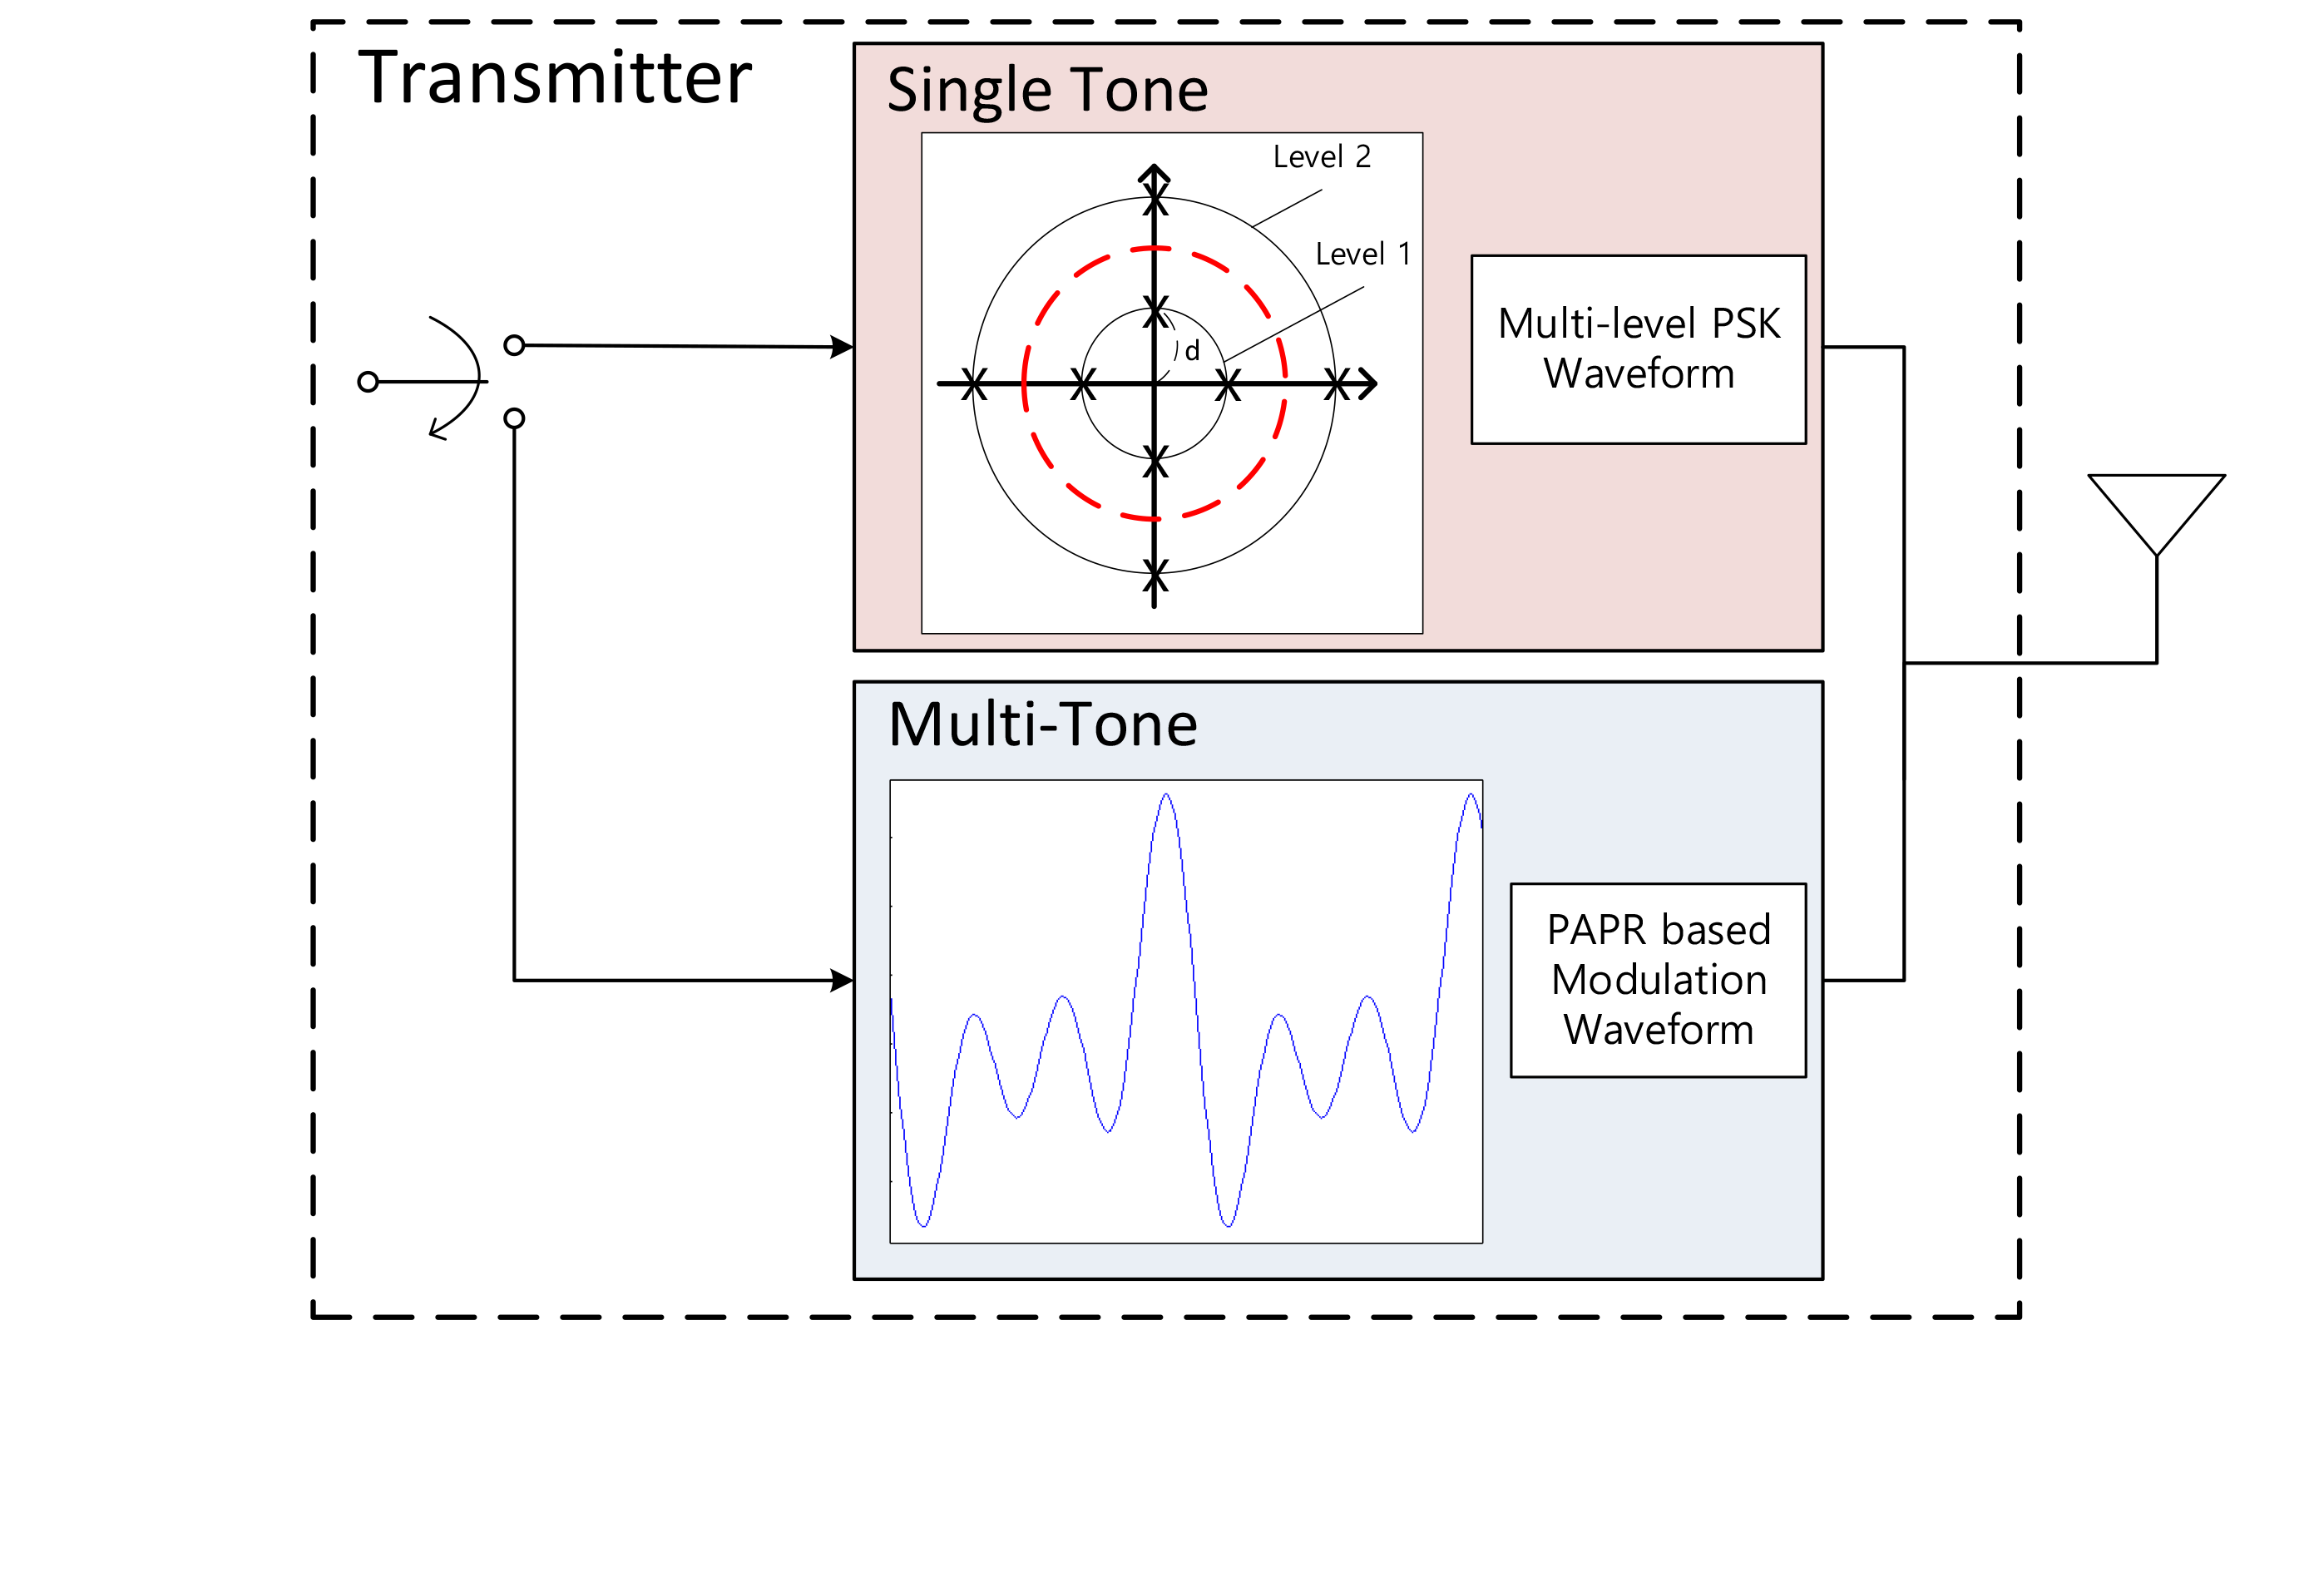
\includegraphics[width=0.45\textwidth]{transmitter}
  \caption{Dual-mode SWIPT transmitter \cite{Park2018}}
  \label{fig:transmitter}
\end{figure}

As shown in Figure \ref{fig:transmitter}, each transmitter consists of a single-tone and a multi-tone signal generator. We will design an adaptive MS algorithm to control the transmission mode according to the received power. The single-tone waveform modulates the amplitude and the phase simultaneously and is suitable for high rate transmission. In contrast, the multi-tone waveform encodes the information by choosing a combination of tones with a specific PAPR level. Therefore, $Q$ tones can be used to transmit ${\log _2}Q$ bits by uniquely mapping to the available subsets. Compared with conventional techniques, the \textit{tone-index multisine modulation} increases the operation range, boosts the harvested power, and reduce the complexity in modulation and demodulation \cite{Krikidis2019}. However, it requires a careful dynamic design to find the tones with high channel gain while keeping the influence of fading on PAPR as low as possible.

\begin{figure}
  \centering
    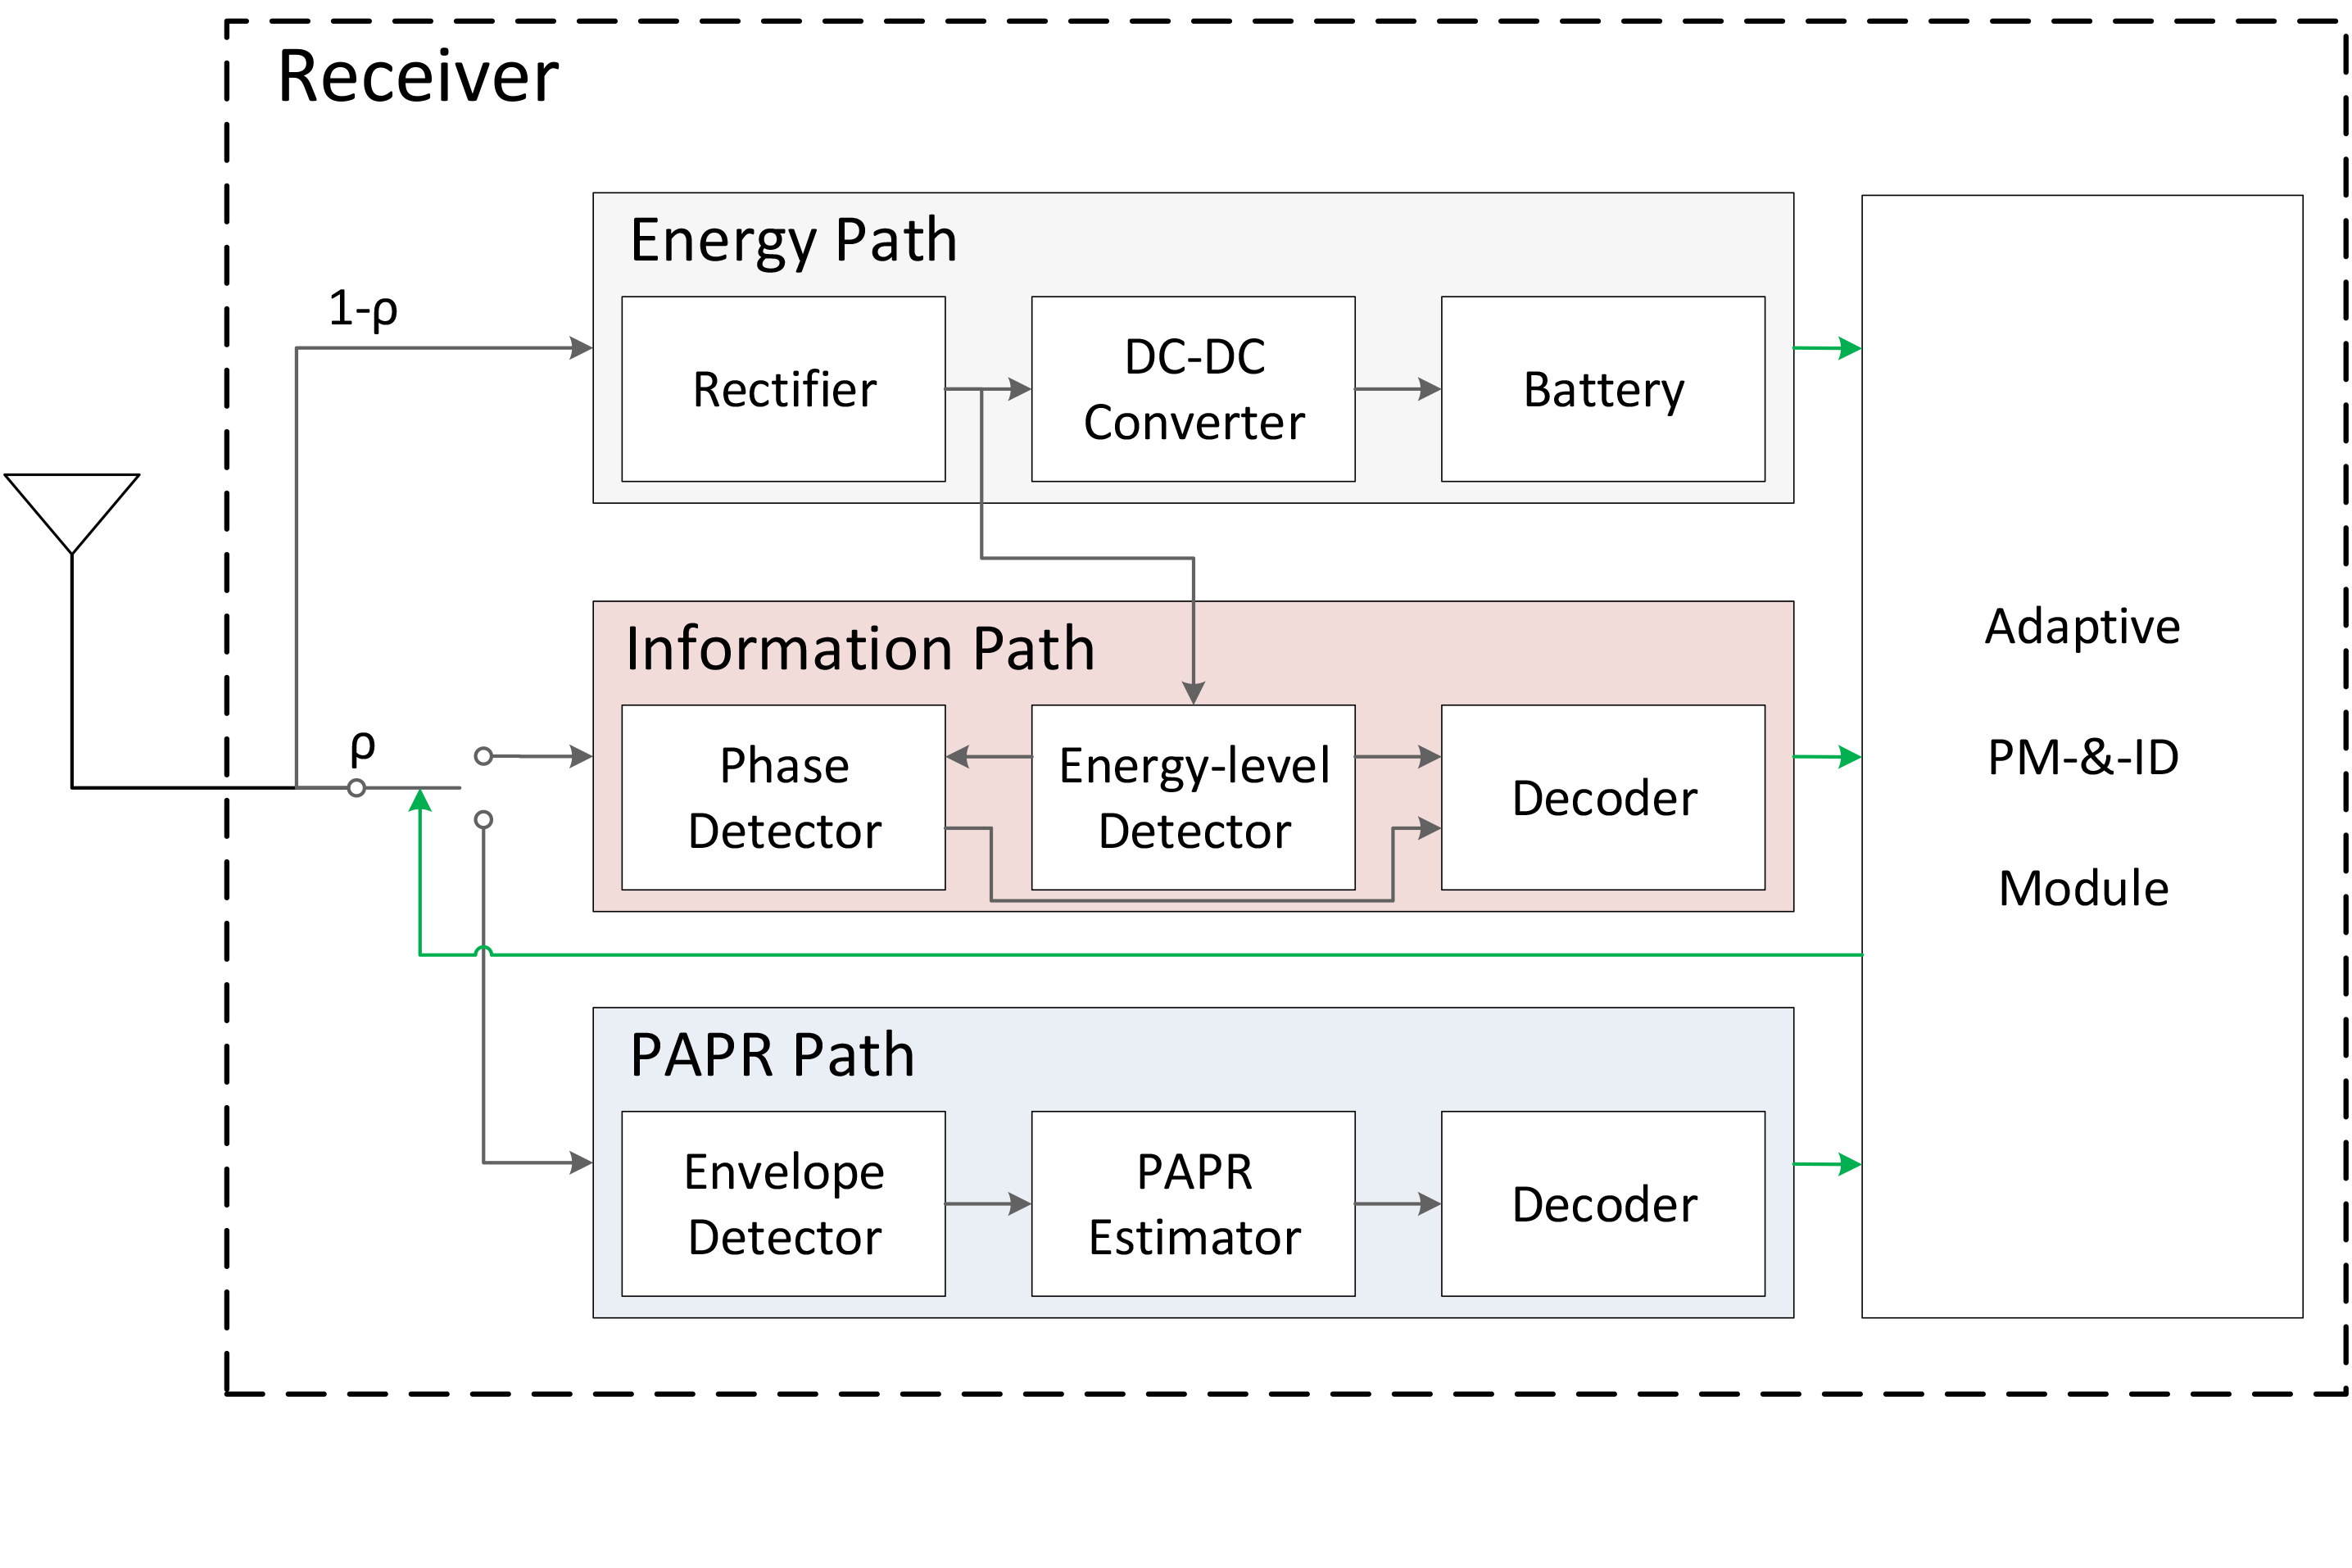
\includegraphics[width=0.45\textwidth]{receiver}
  \caption{Dual-mode SWIPT transmitter \cite{Park2018}}
  \label{fig:receiver}
\end{figure}

The block diagram of an integrated receiver is shown in Figure \ref{fig:receiver}. The \textit{energy paths} in the proposed MIMO multi-harvester system is slightly different from the figure, as we introduce power splitters before the rectifier cluster. With power-information ratio $\rho $, the received signal is divided into energy stream (goes through energy path) and information stream (single-tone goes through information path, multi-tone goes through PAPR path). Note that this ratio is different from the power reallocating ratios that adjust the input power for rectifiers. It is argued in \cite{Park2018} that an infinitesimally small $\rho $ is enough for ID for the property of integrated receiver mentioned in \cite{Zhou2013}. Therefore, most of the received signal can be used for EH. Energy path is used for both power collection and energy-level information decoding. It not only decodes the amplitude information but also transmits the power to \textit{information path} for demodulation. The remaining power will be stored in the battery. Information path estimates CSI then decodes the phase information accordingly. In comparison, \textit{PAPR path} decodes the envelope-based information by measuring the PAPR of the received signal. It does not require channel estimation and active devices, therefore the power consumption is significantly less than information path.

\section{Timeline}
\begin{figure*}
  \begin{ganttchart}[
    expand chart=\textwidth,
    y unit title=0.4cm,
    y unit chart=0.5cm,
    vgrid,hgrid,
    title label anchor/.style={below=-1.6ex},
    title left shift=.05,
    title right shift=-.05,
    title height=1,
    incomplete/.style={fill=white},
    progress label text={},
    bar height=0.7,
    group right shift=0,
    group top shift=.6,
    group height=.3
    group peaks height = .2]{1}{42}
    %labels
    \gantttitle{Year 1}{12}
    \gantttitle{Year 2}{12}
    \gantttitle{Year 3}{12}
    \gantttitle{Year 4}{6} \\

    \gantttitle{Autumn}{3}
    \gantttitle{Winter}{3}
    \gantttitle{Spring}{3}
    \gantttitle{Summer}{3}
    \gantttitle{Autumn}{3}
    \gantttitle{Winter}{3}
    \gantttitle{Spring}{3}
    \gantttitle{Summer}{3}
    \gantttitle{Autumn}{3}
    \gantttitle{Winter}{3}
    \gantttitle{Spring}{3}
    \gantttitle{Summer}{3}
    \gantttitle{Autumn}{3}
    \gantttitle{Winter}{3} \\

    %tasks
    \ganttbar{Courses}{1}{18} \\
    \ganttbar{Literature review}{1}{6} \\
    \ganttbar{Problem formulation}{1}{3} \\
    \ganttbar{Transceiver model design}{7}{9} \\
    \ganttbar{Algorithm development}{10}{15} \\
    \ganttbar{Simulation}{16}{18} \\
    \ganttbar{Result analysis}{19}{21} \\
    \ganttbar{System optimization}{22}{24} \\
    \ganttbar{Expansion and new topics}{25}{42} \\
    \ganttbar{Thesis}{25}{36} \\
    \ganttbar{Proofreading}{37}{42} \\

    %milestones
    \ganttmilestone{Initial research plan}{3} \\
    \ganttmilestone{Early stage review}{9} \\
    \ganttmilestone{Late stage review}{24} \\
    \ganttmilestone{Thesis submission and oral exam}{42}

    %relations
    \ganttlink{elem1}{elem3}
    \ganttlink{elem1}{elem4}
    \ganttlink{elem2}{elem3}
    \ganttlink{elem2}{elem4}
    \ganttlink{elem3}{elem4}
    \ganttlink{elem4}{elem5}
    \ganttlink{elem5}{elem6}
    \ganttlink{elem6}{elem7}
    \ganttlink{elem7}{elem8}
    \ganttlink{elem7}{elem9}
    \ganttlink{elem9}{elem10}

  \end{ganttchart}
 \caption{Gantt chart of the project}
 \label{fig:gantt}
\end{figure*}

The planned timeline is shown in Figure \ref{fig:gantt}.

\section{Discussion}
The proposed design is expected to increase the operation range, guarantee the transmission rate, and provide more power to energy-constrained wireless devices. However, the CSIT acquisition with nonlinear models is challenging and the power splitting ratios are difficult to change dynamically. Although the research on SWIPT is still in the theoretical stage and the harvester nonlinearity brings coupling in the system design, I believe it is a key-enabling technique for future wireless networks and would love to contribute to the innovation.

My interest in this specific topic emerged when I was doing MSc project on SWIPT \href{https://github.com/SnowzTail/signal-optimization-for-wireless-information-and-power-transmission}{[link]}. It was a signal design following \cite{Clerckx2018} where a superposition of information (modulated) and power (multisine) waveforms are jointly optimized with power splitting ratio according to the CSI. The iterative algorithms are based on non-convex posynomial maximization. It is sensitive to initialization and may take a long time to converge for multi-subband transmission. As an alternative, the dual-mode SWIPT in \cite{Park2018} reduces the complexity by switching between PSK and PAPR modulation to ensure high power level. The idea of encoding and decoding using PAPR is very interesting, but the performance deserves further study especially for FS channels. Moreover, the harvester model in the previous project was based on the Taylor series approximation of the diode characteristic equation \cite{Clerckx2016}, but both \cite{Park2018} and \cite{Ma2019} employed a logistic curve fitting technique proposed in \cite{Boshkovska2015} that I would like to investigate.

\section{Ethics}
There are no ethical issues involved in this project.

\bibliographystyle{IEEEtran}
\bibliography{library}

\end{document} 